\section{Systemsoftware f"ur Mesh-Netzwerk}

In Kapitel 4 haben wir mehrere Hardware-L"osungen f�r ein Mesh-Netztwerk
vorgestellt. F"ur alle im Kapitel 4 vorgestellten PCI-, MiniPCI- und
PCMCIA-Karten werden vom Hersteller dieser WLAN-Karten Windows-Treiber
bereitgestellt. Und nur wenige Hersteller (z.B. Intel) haben auch Linux-Treiber
f"ur ihre Karten implementiert. Gl"ucklicherweise existiert f"ur
WLAN-Karten mit Atheros-Chipsatz der Open-Source Linux-Treiber MadWifi,
der alle im Kapitel 4 aufgelisteten WLAN-Karten mit Atheros-Chipsatz
unterst"utzt. Bei Soho-Routern sieht die Situation etwas anders aus. Hier gibt
es nicht so viele M"oglichkeiten bei der Wahl nach einer Software.
Die meisten Hersteller von SoHo-Routern stellen den Source-Code des
Betriebssystems f"ur SoHo-Router nicht bereit. Deswegen wird eine
Open-Source Firmware gebraucht, mit der SoHo-Router im Ad-Hoc Modus
betrieben werden k"onnen, denn die meisten SoHo-Router arbeiten nur
im Infrastruktur Modus und den Ad-Hoc Modus nicht realisieren.

In diesem Kapitel wird verschiedene Treiber- und Routing-Software
vorgestellt, die zusammen mit der Hardware aus Kapitel 4 die Realiesierung
von Ad-Hoc Mesh-Netzwerken erm"oglicht.

\subsection{Linux MadWiFi-Treiber}

Linux MadWifi-Treiber \cite{madwifi} ist Linux Kernel Treiber f"ur
WLAN-Karten mit
Atheros Chipsatz. Linux MadWifi-Treiber ist heutzutage einer der
fortgeschrittensten Linux Treiber f"ur WLAN-Karten. Der Treiber ist stabil
und hat eine gro"se Benutzergemeinschaft. Der MadWifi-Treiber selbst ist
Open-Source, verwendet aber eine proprit�re Softwareschicht Hardware
Abstraction Layer (HAL), die nur in bin"arer Form vorhanden ist.

Das Hardware Abstraction Layer (HAL) wird vom MadWifi-Treiber gebraucht,
um die Atheros-Chips ansprechen zu k"onnen. Daf"ur wurde bisher ein
Closed-Source-Modul verwendet. Dies hat unter anderem damit zu tun,
dass die Atheros-Chips"atze prinzipiell auf Frequenzen funken k"onnten,
f"ur die sie nicht zugelassen sind - beispielsweise weil diese vom Milit"ar
zur Kommunikation verwendet werden.

Durch das propriet"are Modul war der Madwifi-Treiber bisher jedoch von
einer Aufnahme in den Linux-Kernel ausgeschlossen. Die Entwickler hatten
au"serdem das Problem, dass sie Fehler unter Umst"anden nicht beheben
konnten, da sie nicht nachvollziehen konnten, wie der HAL-Baustein
arbeitet.

MadWifi selbst wird daher ab sofort nicht weiterentwickelt. Stattdessen
setzen die Programmierer auf OpenHAL, eine Linux-Portierung des
HAL-Modules des in OpenBSD verf"ugbaren freien Atheros-Treibers. In der
Vergangenheit wurde vom Software Freedom Law Center (SFLC) best"atigt,
dass die durch Reverse Engineering entstandene Software keine Copyrights
verletzt. Solche Behauptungen hatten die Entwicklung lange ausgebremst.

Der neue Treiber "`Ath5k"' wird MadWifi nun ersetzen und soll nicht nur
die freie Komponente OpenHAL einsetzen, sondern auch mit dem neuen
Linux-WLAN-System Mac80211 zusammenarbeiten, so dass der Treiber in den
offiziellen Linux-Kernel gelangen kann. MadWifi soll jedoch weiter mit
Fehlerkorrekturen und HAL-Updates versorgt werden.

\textbf{Links:}

\begin{itemize}
\item \url{http://madwifi.org/}
\item \url{http://madwifi.org/wiki/About/ar5k}
\item \url{http://madwifi.org/wiki/About/OpenHAL}
\item \url{http://madwifi.org/wiki/UserDocs/GettingMadwifi}
\item \url{http://madwifi.org/wiki/Compatibility}
\item \url{http://www.intellinuxwireless.org/?p=mac80211}
\end{itemize}

\subsection{Open-Source Firmware f"ur SoHO WLAN-Router}
\label{sec:Open-Source Firmware f"ur SoHO WLAN-Router}

In diesem Abschnitt werden mehrere Open-Source Firmwares f"ur SoHO WLAN-Router
vorgestellt. Diese Firmwares werden gebraucht, damit man SoHO WLAN-Router
im Ad-Hoc Modus betreiben kann, denn die meisten SoHO WLAN-Router unterst"utzen
nur WLAN Infrastruktur Modus. Alle unten erw"ahnten Firmwares basieren
auf dem Quellcode des Betriebssystems des Linksys WRT54G SoHO WLAN-Router.

\subsubsection{OpenWRT}

OpenWRT ist eine GNU/Linux-Distribution f"ur WLAN-Router.
OpenWRT l"auft unter anderem auf Ger"aten der Firmen Linksys, ALLNET,
ASUS, Belkin, Buffalo, Microsoft und Siemens \cite{openwrt}.

\subsubsection{DD-WRT}

DD-WRT ist eine GNU/Linux-Distribution f"ur WLAN-Router.
DD-WRT untest"utzt Ger"ate Firma Linksys, z.B. WRT54G und
WRT54GS bis Version 4.x. Es werden aber inzwischen auch Ger"ate anderer
Hersteller unterst�tzt (z. B. Buffalo, Siemens, Asus, Belkin)
\cite{dd-wrt}.

\subsubsection{FreeWRT}

FreeWRT ist eine GNU/Linux-Distribution f"ur WLAN-Router.
FreeWRT unterst"utzt nur Systeme mit Broadcom Ger"aten, z.B.
Linksys WRT54GL, Asus WL500g Premium und Netgear WGT634u
\cite{freewrt}.

\subsection{Mesh-Routing Software}

In diesem Abschnitt werden Routing-Deamonen vorgestellt, die ein
bestimmtes Routing-Protokoll implementieren und auf jedem Knoten in
einem Mesh-Netzwerk ausgef"uhrt werden. Diese Daemonen tauschen
Routing-Informationen aus und machen es m"oglch, Nachrichten
von einem Knoten zu einem anderen Knoten im Mesh-Netzwerk zu
transportieren. Routing-Daemonen erm"oglichen die Kommunikation zwischen
2 Knoten in einem Ad-Hoc Mesh-Netzwerk, zwischen denen mehr als 1 Hop
liegt.

\subsubsection{olsr.org OLSR daemon}


\includegraphics{Olsrd_logo.png}

Der olsr.org OLSR daemon \cite{olsrd} ist eine Implementierung des Optimized Link
State Routing Protokolls. OLSR ist ein Routing-Protokoll f"ur mobile Ad-Hoc
Netzwerke. Der Protokoll ist pro-aktiv, tabellengesteuert und nutzt die
Technik Multipoint Relaying (MPR) zum Fluten von Nachrichten. olsrd
implementiert ausserdem auch eine popul"are Erweiterung Link Quality
Extension. Zur Zeit ist die Implementierung von olsrd verf"ugbar f�r
GNU/Linux, Windows, OS X, FreeBSD, OpenBSD and NetBSD. olsrd ist eine
gut strukturierte und kodierte Implementierung, die leicht zu warten,
zu erweitern und auf andere Plattforme zu portieren sein soll. Die
Implementierung ist konform zu RFC3626 in Bezug auf die Kernfunktionalit"at
und die zus"atzlichen Funktionen. olsrd unterst"utz das Konzept von ladbaren
Plug-Ins. Mit diesen Plug-Ins kann man benutzerdefinierte Pakete mit
Hilfe des OLSR MPR Flutens versenden und behandeln oder irgendeine andere
zus"atzliche Funktionalit"at bereitstellen.

Links:
\begin{itemize}
\item \url{http://ietf.org/rfc/rfc3626.txt}
\item \url{http://wiki.freifunk.net/OLSR\_mit\_Windows}
\item \url{http://wireless.subsignal.org/index.php?title=Laptop\_mit\_OLSR}
\item \url{http://wiki.opennet-initiative.de/index.php/OLSR}
\end{itemize}

\subsubsection{Open-Mesh B.A.T.M.A.N. daemon}

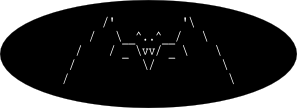
\includegraphics{Batman_logo.png}

Der B.A.T.M.A.N.-Daemon \cite{batman} steht bislang f"ur Linux, FreeBSD und Macintosh
OS-X zur Verf"ugung. Die Entwicklungsarbeit konzentriert sich jedoch
in erster Linie auf Linux, weshalb es vorkommen kann, dass erweiterte
Funktionen unter anderen Betriebssystemen erst mit einer gewissen
Verz"ogerung zur Verf"ugung stehen.

Linux-Installationspakete des B.A.T.M.A.N.-Daemon batmand gibt es f"ur
Debian, OpenZaurus und OpenWRT. Zum Kompilieren aus dem Quelltext gen�gt
ein einfaches make und make install im Sourcecodeverzeichnis. Als einzige
Abh"angigkeit wird die Bibliothek libpthread vorausgesetzt, die auf einem
Linux-System, "ublicherweise bereits installiert sein sollte.

Um "uber ein B.A.T.M.A.N.-Mesh ins Internet gehen zu k"onnen, muss
au"serdem unter Linux das Kernelmodul tun installiert sein. Es ist
im Standardkernel der meisten Linuxdistributionen enthalten und wird beim
ersten Start des B.A.T.M.A.N.-Daemons automatisch geladen. Wer einen
selbstkompilierten Kernel einsetzt, findet es zum Beispiel in xconfig
in der Abteilung Network Device Support unter der Bezeichnung Universal
TUN/TAP device driver support.

Links:
\begin{itemize}
\item \url{https://www.open-mesh.net/Members/adagio/batman-install-howto-stichworte}
\item \url{http://open-mesh.net/batman/doc/batmand\_howto.pdf}
\item \url{https://www.opensourcepress.de/fileadmin/osp/pdf/mesh\_leseprobe.pdf}
\end{itemize}

\subsubsection{Meshcom Driver}


\includegraphics{meshcomlogo.png}

Der MeshDriver klemmt sich zwischen den WLAN-Treiber und den
TCP/IP-Stack. Anders als 802.11s funkt er im Ad-hoc-Modus von 802.11 und
bezieht eine Ethernet-Schnittstelle automatisch in das vermaschte Netz
ein, etwa f"ur den Internet-Zugang. Meshcom stellt eine Beta-Version
f"ur privaten Einsatz und Forschungszwecke kostenlos zur Verfugung,
die unter Windows XP oder Linux mit Kernel 2.6 lauft. Sie beherrscht
allerdings einige wesentliche Features noch nicht, beispielsweise
Authentifizierung und Verschl"usselung. Auch reaktives Routing fehlt noch,
also das fallweise Bestimmen der Route an Stelle von vorab festgelegten
Routing-Tabellen.

Links:
\begin{itemize}
\item \url{http://www.meshcom.com/}
\end{itemize}

